\section{Second modèle}
\label{sec:SecondModel}

En reprenant le modèle exposé en partie \ref{sec:PremierModel}, 
nous changeons maintenant d'objectif. On souhaite à présent, à partir d'une
suite d'accords, trouver une suite de positions physiquement jouables
minimisant une certaine fonction de poids.\\
On a constaté deux choses, d'abord qu'il est assez fastudieux de déclarer des
contraintes sur nos variables, d'autre part que l'ensemble des possibles
parcouru par le solver est grand. Pour un accord, il est de
$\nbCordes^\nbFrettes$ et donc pour une suite d'accords il est de
$\nbAccord^{\nbCordes^\nbFrettes}$, cela fait beaucoup et nous allons raffiner 
l'ensemble des possibles.

Nous optons pour une approche en extension du problème. C'est à dire que l'on 
va filtrer les solutions possibles pour tendre vers une résolution plus 
efficace.

\subsection{Filtrage, contraintes en extensions et principe du MDD}
\label{subsec:Extension}

Le filtrage permet de restreindre l'ensemble de recherche. Par exemple, on peut
rechercher une solution à notre problème dans l'ensemble des positions
possibles (de cardinal $\nbCordes^{\nbFrettes}$), ou dans l'ensemble des positions physiquement possibles (de cardinal
$\posiPhyPos$). C'est là le premier filtrage que l'on a effectué.

\begin{figure}[H]
  \centering
  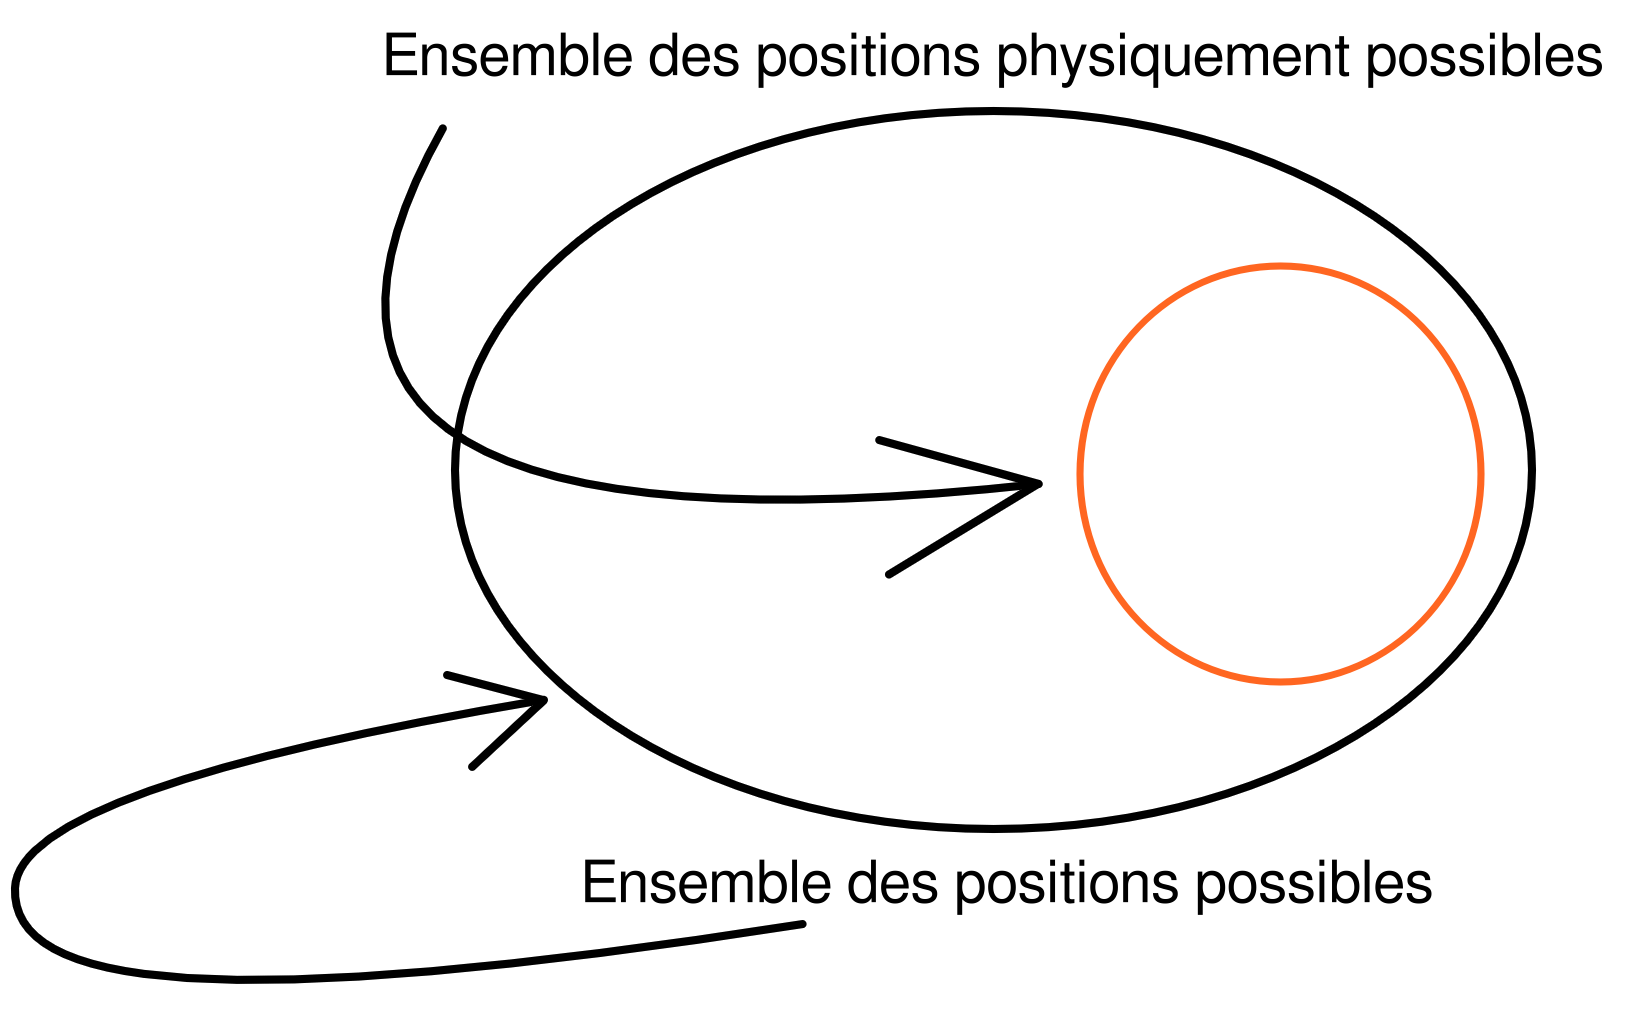
\includegraphics[width=0.4\textwidth]{images/ensembles/ensemble1.png}
  \caption{Représentation du filtrage}
  \label{fig:ensemble1}
\end{figure}

Comme indiqué dans la figure \ref{fig:ensemble1}, en parcourant l'ensemble des 
positions et en les filtrant nous allons passer d'un espace de recherche
de $\nbAccord^{\nbCordes^{\nbFrettes}}$ à $\nbAccord^{\posiPhyPos}$.\\
Pour ce faire, on va réaliser une table des positions physiquement possibles.\\
Pour cela, on parcourt l'ensemble des positions et l'on vérifie pour chacune
si elle est physiquement jouable voir code \ref{code:parcoursFiltrage}.
Ici on a enrichi la notion de physiquement jouable, en effet, il n'est plus
question que de distance entre les doigts mais aussi de la possibilité de
réaliser des barrés ainsi que du nombre de doigts utilisés.

\begin{figure}[H]
  \begin{lstlisting}[language=Java]
Tuples positions_legales = new Tuples(true);
for (int i=0; i<(int)Math.pow((double)nf, (double)(nc+1)); i++)
{
	int[] position_courante = new int[nc];
	for (int j=0; j<nc; j++)
	{
		position_courante[j]=(i/((int)Math.pow((double)nf, (double)j))%nf)-1;	
	}
	if (est_legal(position_courante, nc, nf, distanceFirstFrette, barre, nbDoigts))
	{
    positions_legales.add(position_courante);
	}
}
\end{lstlisting}
  \caption{Parcours de l'ensemble des positions et filtrage en fonction de la
  jouabilité}
  \label{code:parcoursFiltrage}
\end{figure}

Une fois cette table établie, on va créer un modèle de contraintes où les
indéterminées seront les suites de positions.
L'avantage ici par rapport à la permière partie est que le solver ne parcourt 
pas un arbre des possibles trop grand, mais qu'on calcule une fois un sous
arbre pertinent. Pour ce calcul on parcour effectivement l'ensemble des
positions sur la guitare, mais d'une part on le réalise qu'une fois et non pas
une fois par accords, et c'est un calcul beaucoup moins couteux que celui du
solver.

Les tuples implémentés dans choco utilisent une structure efficace en temps et
en espace : c'est la structure de MDD. 
On va un peu développer sur ce qu'est le MDD et montrer pourquoi c'est efficace.

Pour définir ce qu'est un MDD et pour montrer son intérêt, j'utilise un article
de G.Perez et J.C.Régin \cite{PerezR16}.

\begin{defi}(MDD)
  \label{def:MDD}
  Un multi-valued decision diagram (MDD), est une structure de données qui
  représente des fonctions discrètes. Dans le cadre de la PPC, on utilise les
  MDD pour représenter des fonctions de la forme 
  $f : \accolades{0\dots d-1}^r \rightarrow 
  \accolades{true, false}$.\\
  La structure de données prend la forme d'un graphe composé de $r$ couches.
  Les couches sont des ensembles d'arcs de même profondeur.
  , et
  sur chacune des couches les noeuds possèdent au plus $d$ arcs sortants allant
  à la couche d'après. La couche finale représente le noeud acceptant du MDD.
  Chaque arc  les variables. Un tuple est accepté par
  un MDD \ssi il existe dans le graphe un chemin de la première à la dernière
  couche tel que l'étiquette de l'arc à la couche $i$ soit la $i$ valeur du
  tuple.
\end{defi}

%-----------------------------

Voici un exemple pour illustrer la definition \ref{def:MDD} :
\begin{figure}[H]

\centering
\begin{subfigure}{0.4\textwidth}
  \begin {tikzpicture}[-latex ,auto ,node distance =3cm ,on grid ,
  semithick ,
  state/.style ={ circle ,top color =white , bottom color = processblue!20 ,
  draw,processblue , text=black , minimum width =0.5 cm}]
  \node[state] (A) {$ff$};
  \node[state] (B) [above left=of A] {$1$};
  \node[state] (C) [above right =of A] {$2$};
  \node[state] (D) [above right=of B] {$0$};
  \path (D) edge node {a} (B);
  \path (D) edge node {c} (C);
  \path (B) edge [bend right =35] node {a} (A);
  \path (B) edge [bend left =35] node {b} (A);
  \path (C) edge [bend left =35] node {a} (A);
  \path (C) edge node {b} (A);
  \path (C) edge [bend right =35] node {c} (A);
  \end{tikzpicture}
  \caption{MDD}
\end{subfigure}
\hfill
\begin{subfigure}{0.55\textwidth}
  \begin {tikzpicture}[-latex ,auto ,node distance =2.3cm ,on grid ,
  semithick ,
  state/.style ={ circle ,top color =white , bottom color = processblue!20 ,
  draw,processblue , text=black , minimum width =0.5 cm}]
  \node[state] (A1) {$3$};
  \node[state] (A2) [right=of A1] {$4$};
  \node[state] (A3) [right=of A2] {$5$};
  \node[state] (A4) [right=of A3] {$6$};
  \node[state] (A5) [right=of A4] {$7$};
  \node[state] (B2) [above=of A2] {$2$};
  \node[state] (C) [above =of A4] {$3$};
  \node[state] (D) [above right=of B2] {$0$};
  \path (D) edge node {b} (B2);
  \path (D) edge node {c} (C);
  \path (B2) edge node {a} (A1);
  \path (B2) edge node {b} (A2);
  \path (C) edge node {a} (A3);
  \path (C) edge node {b} (A4);
  \path (C) edge node {c} (A5);
  \end{tikzpicture}
  \caption{Arbre}
\end{subfigure}
\caption{Les deux graphes (MDD et arbre) représentent les tuples
$\accolades{\accolades{a,a},\accolades{a,b},\accolades{c,a},\accolades{c,b},\accolades{c,c}}$}
\end{figure}

Les intérêts d'un MDD est qu'il est rapide de déterminer si un tuple appartient
à la table qu'il décrit et qu'il prend peu de place en espace comparativement
à un arbre.
En effet, les sommets et arcs d'un MDD sont fusionnés de sorte à ce qu'il 
prenne le moins de place possible. De plus, la vérification de la validité 
d'un tuple se fait en la profondeur et donc linéairement en la taille du tuple.
Les algorithmes pour transformer un ensemble de tuples en MDD sont déjà
implémentés dans choco.\\
Une fois que l'on a créé la table on ajoute des contraintes de tables, 
c'est à dire que l'on réduit le domaine de la position aux positions 
physiquement jouables.

Dans la recherche de solution, on indique au solver une fonction à minimiser.
Ainsi, choco va trouver une solution au problème qui est minimale pour la 
fonction indiquée. Nous dédierons la sous partie 
\ref{subsubsec:funMinimisation} à cette fonction de 
minimisation qui prend en compte les attentes de l'instrumentiste.

On peut alors tester notre programme sur différentes suites d'accords.\\
On observe que le programme fonctionne bien pour une suite de $4$ accords, on
obtient une solution en moins de $4$ secondes, mais pour une suite de $6$ 
accords l'algorithme met déja plus longtemps ($\sim 20$sec), et pour 10 accords
($\geq20$min) ce qui n'est pas acceptable. Il faut améliorer le temps de
recherche.

\subsection{Stratégie de recherche}
\label{subsec:strategie}

Pour un parcours exhaustif, on a $\nbAccord^{\posiPhyPos}$
possibilités. Ce qui reste relativement grand.

Un première optimisation est de définir une stratégie de recherche dans le 
graphe des possibles.
La stratégie de recherche consiste à indiquer au solver l'ordre des positions
à fixer en premier.
Elle permet d'éliminer des mauvais candidats et d'éviter 
de parcourir toutes les potentielles solutions. En effet, si l'on a trouvé une
solution de poids $p$ et qu'au cours de la recherche d'une solution (de la
première position à la dernière position) on obtient un poids partiel $p'>p$
sur un accord intermédiaire, on stoppe la recherche pour ce candidat partiel.
\begin{figure}[H]
  \centering
  \begin {tikzpicture}[-latex ,auto ,node distance =3cm ,on grid ,
  semithick ,
  state/.style ={ circle ,top color =white , bottom color = processblue!20 ,
  draw,processblue , text=black , minimum width =0.5 cm}]


  \node[state] (AA) at (0,3) {$1$};
  \node[state] (AB) at (0,1) {$2$};
  \node (TPAA) at(0,-0.6) [draw, rectangle, color=white, text=black] {.};
  \node (TPAB) at(0,-0.8) [draw, rectangle, color=white, text=black] {.};
  \node (TPAC) at(0,-1) [draw, rectangle, color=white, text=black] {.};
  \node[state] (AC) at (0,-2.4) {$n_1$};
  \node (TA) at (0,-3.5) [draw = white, rectangle, text = black] {Prem.posi.};

  \node[state] (BA) at (3,3) {$1$};
  \path[cyan] (AA) edge node {} (BA);
  \path (AB) edge node {} (BA);
  \path (AC) edge node {} (BA);
  \node[state] (BB) at (3,1) {$2$};
  \path (AA) edge node {} (BB);
  \path (AB) edge node {} (BB);
  \path (AC) edge node {} (BB);
  \node (TPBA) at(3,-0.6) [draw, rectangle, color=white, text=black] {.};
  \node (TPBB) at(3,-0.8) [draw, rectangle, color=white, text=black] {.};
  \node (TPBC) at(3,-1) [draw, rectangle, color=white, text=black] {.};
  \node[state] (BC) at (3,-2.4) {$n_2$};
  \path[red] (AA) edge node {} (BC);
  \path (AB) edge node {} (BC);
  \path (AC) edge node {} (BC);
  \node (TB) at(3,-3.5) [draw = white, rectangle, text = black] {Sec.posi.};
 
  \node[state] (CA) at (6,3) {$1$};
  \path (BA) edge node {} (CA);
  \path (BB) edge node {} (CA);
  \path (BC) edge node {} (CA);
  \node[state] (CB) at (6,1) {$2$};
  \path (BA) edge node {} (CB);
  \path (BB) edge node {} (CB);
  \path[red] (BC) edge node {} (CB);
  \node (TPCA) at(6,-0.6) [draw, rectangle, color=white, text=black] {.};
  \node (TPCB) at(6,-0.8) [draw, rectangle, color=white, text=black] {.};
  \node (TPCC) at(6,-1) [draw, rectangle, color=white, text=black] {.};
  \node[state] (CC) at (6,-2.4) {$n_3$};
  \path[cyan] (BA) edge node {} (CC);
  \path (BB) edge node {} (CC);
  \path (BC) edge node {} (CC);
  \node (BB) at(6,-3.5) [draw = white, rectangle, text = black] {Tro.posi.};
  
  \node (PR) at(7.5, 1) [draw = white, rectangle, text = red] {poids : 20};

  \node (TP) at(8,0) [draw = white, rectangle, text=black] {. . .};

  \node[state] (PNA) at (10,3) {$1$};
  \node[state] (PNB) at (10,1) {$2$};
  \node (TPPNA) at(10,-0.6) [draw, rectangle, color=white, text=black] {.};
  \node (TPPNB) at(10,-0.8) [draw, rectangle, color=white, text=black] {.};
  \node (TPPNC) at(10,-1) [draw, rectangle, color=white, text=black] {.};
  \node[state] (PNC) at (10,-2.4) {$n_{m-1}$};
  \node (TB) at(10,-3.5) [draw = white, rectangle, text = black] {Av.der.posi.};

  \draw[cyan, densely dotted, ->] (CC) to[out=45, in=225, looseness=1.5] (PNB);
  
  \node[state] (NA) at (13,3) {$1$};
  \path (PNA) edge node {} (NA);
  \path (PNB) edge node {} (NA);
  \path (PNC) edge node {} (NA);
  \node[state] (NB) at (13,1) {$2$};
  \path (PNA) edge node {} (NB);
  \path[cyan] (PNB) edge node {} (NB);
  \path (PNC) edge node {} (NB);
  \node (TPNA) at(13,-0.6) [draw, rectangle, color=white, text=black] {.};
  \node (TPNB) at(13,-0.8) [draw, rectangle, color=white, text=black] {.};
  \node (TPNC) at(13,-1) [draw, rectangle, color=white, text=black] {.};
  \node[state] (NC) at (13,-2.4) {$n_m$};
  \path (PNA) edge node {} (NC);
  \path (PNB) edge node {} (NC);
  \path (PNC) edge node {} (NC);
  \node (TB) at(13,-3.5) [draw = white, rectangle, text = black] {Der.posi.};
  
  \node (PR) at(14.5, 1) [draw = white, rectangle, text = cyan] {poids : 15};
  \end{tikzpicture}
  \caption{Représentation d'élagage obtenu par la stratégie de recherche dans\\ 
  un ensemble de $m$ positions avec $n_i$ positions possibles 
  pour la $i^{\text{ème}}$ indéterminée}
  \label{fig:stratRech}
\end{figure}
Dans la figure \ref{fig:stratRech}, la stratégie de recherche va parcourir les
positions possibles des tables de gauche (premier accord) à droite (dernier
accord) en calculant le poids peu à peu et élimine les chemins de poids
supèrieurs à ceux déja calculé. 
Par exemple, après avoir parcouru le chemin bleu et calculé son
poids, le solver parcours, le chemin rouge et obtient en cours de parcours un
poids superieur au chemin bleu qui est complet. Sachant que le poids est une
fonction croissante car dans la fonction de calcul on n'a pas de poids negatif,
le solveur arrête la recherche après la section de chemin rouge. 
Cela permiet de réaliser un élagage de l'ensemble de recherche.

Par exemple, on réalise le programme sans et avec une stratégie de résolution
sur des entrées de tailles différentes avec comme fonction à minimiser une
fonction qui est minimale quand les positions sont vers le haut du manche de la
guitare (et donc que les positions sont proche de $0$):

\begin{figure}[H]
%\begin{center}
  \centering
  \begin{tabular}{||c c c||}
    \hline
    Nombre d'accords & Sans & Avec \\ [0.5ex]
    \hline\hline
    $4$ & $2$s & $2$s \\
    \hline
    $5$ & $6$s & $3$s \\
    \hline
    $6$ & $20$s & $4$s \\
    \hline
    $10$ & $\geqslant20$min & $38$s\\[1ex]
    \hline
  \end{tabular}
%\end{center}
\caption{Tableau comparatif du temps d'execution en fonction du nombre\\
  d'accords de la suite avec et sans la stratégie de recherche}
\label{tab:compSR}
\end{figure}

On peut voir dans le tableau \ref{tab:compSR} que la stratégie de recherche est
très efficace. Mais cela s'explique en partie par l'objectif de minimisation et
par la suite d'accords utilisés (ici les $4$ premiers accords de Let It Be
joués en boucle). La stratégie de recherche peut s'avérer plus ou moins
efficace en fonction de la suite d'accords.

\subsection{SAC}
\label{subsec:SAC}

Une méthode d'optimisation par prétraitement conseillée par Charles est celle 
de la SAC (singleton arc consistency). 
Charles a développé une classe choco permettant d'appliquer quelques stratégies 
de prétraitement que j'ai pu tester dans le cadre de mon stage.
Nous allons détailler ce qu'est la SAC et comment le processus permet au
programme de gagner en efficacité. Pour définir le principe de SAC, on s'appuie 
sur le chapitre \cite{BESSIEREsac}.

On pose $$N = \left(\mathcal{X}, \mathcal{D}, \mathcal{C}\right)$$ une instance
du problème.

\begin{defi}(Consistance)
  Soit $v_i\in\domaine(x_i)$,\\
  $v_i$ est consistante avec $c\in\contr$ \ssi il existe une valuation
  $\tau$ vérifiant $c$ tel que $\tau\left[x_i\right]=v_i$.
\end{defi}

\begin{defi}(Arc-Consistant)
  Soit $c\in\contr$,\\
  $\domaine$ est arc-consistant sur $c$ pour
  $x_i\in\indet$ \ssi pour tout $v_i\in\domaine(x_i)$, $v_i$ est
  consistante avec $c$ dans $\domaine$.
  On dit de $N$ qu'il est arc-consistant \ssi 
  pour tout $x\in\indet$, $\domaine$ est
  arc consistant pour $x$ sur toute contrainte $c$ de $\contr$.
\end{defi}

\begin{defi}(Arc-Inconsistant)
  $N$ est arc-inconsistant \ssi l'ensemble vide est l'unique domaine strictement
  plus petit que $\domaine$ qui est arc-consistant pour toutes variables,
  sur toutes contraintes.
\end{defi}

\begin{defi}(Singleton Arc Consistant)
  $N$ est singleton arc consistant (SAC) \ssi pour toute indéterminée
  $x_i\in\indet$ et pour toute valeur $v_i\in\domaine(x_i)$, le sous
  problème $\restr{N}{x_i=v_i}$ n'est pas arc inconsistant.
\end{defi}

Un modèle qui est singleton arc consistant est un modèle pour lequel les
domaines sont minimaux, dans le sens où il n'existe pas de valuations qui
ne vérifie pas l'ensemble des contraintes.
Transformer un modèle en modèle SAC permet donc de réduire ses domaines et
d'avoir un espace de recherche restreint.
Par exemple, transformer le modèle étudié dans cette partie en modèle SAC 
garantit que le domaine de l'indéterminée de la première position comporte 
uniquement des positions du premier accord.
Sans la SAC, si le premier accord est un do majeur (do, mi, sol), 
une position avec la deuxème corde à vide (la) aurait été présente dans les
domaines, alors qu'avec la sac, une position dans laquelle un la est joué 
va à l'encontre de la contrainte d'accord et n'apparaît pas dans les domaines.
Ainsi, en réalisant un préprocessing, le solver choco raffine les domaines. 
Une fois le préprocessing effectué, la résolution du problème est beaucoup plus
rapide. Il y a certes un temps de préprocessing mais il n'impacte pas le 
gain de temps pour la résolution.

\subsection{Affiner le filtrage des accords}
\label{subsec:Affinage}

Après discussion avec Charlotte et Charles, nous avons conclu que si la SAC
est performante, c'est que l'ensemble des domaines peut-être mieux décrit dans
la modélisation du problème.

On va donc améliorer la fonction de filtrage. Au lieu de filtrer toutes les
positions physiquement jouables, on va créer une table de hashage qui à chaque 
accord de la suite associe un MDD représentant un ensemble de positions 
autorisées.
Lors du filtrage, à chaque position calculée, si elle est physiquement jouable 
et si elle correspond à un accord de la suite étudiée, on l'ajoute dans le MDD 
associé à cet accord. On obtient alors autant de tables que d'accords 
différents dans lesquels sont stockés uniquement les accords physiquement 
jouables du bon accord.

\begin{figure}[H]
  \centering
  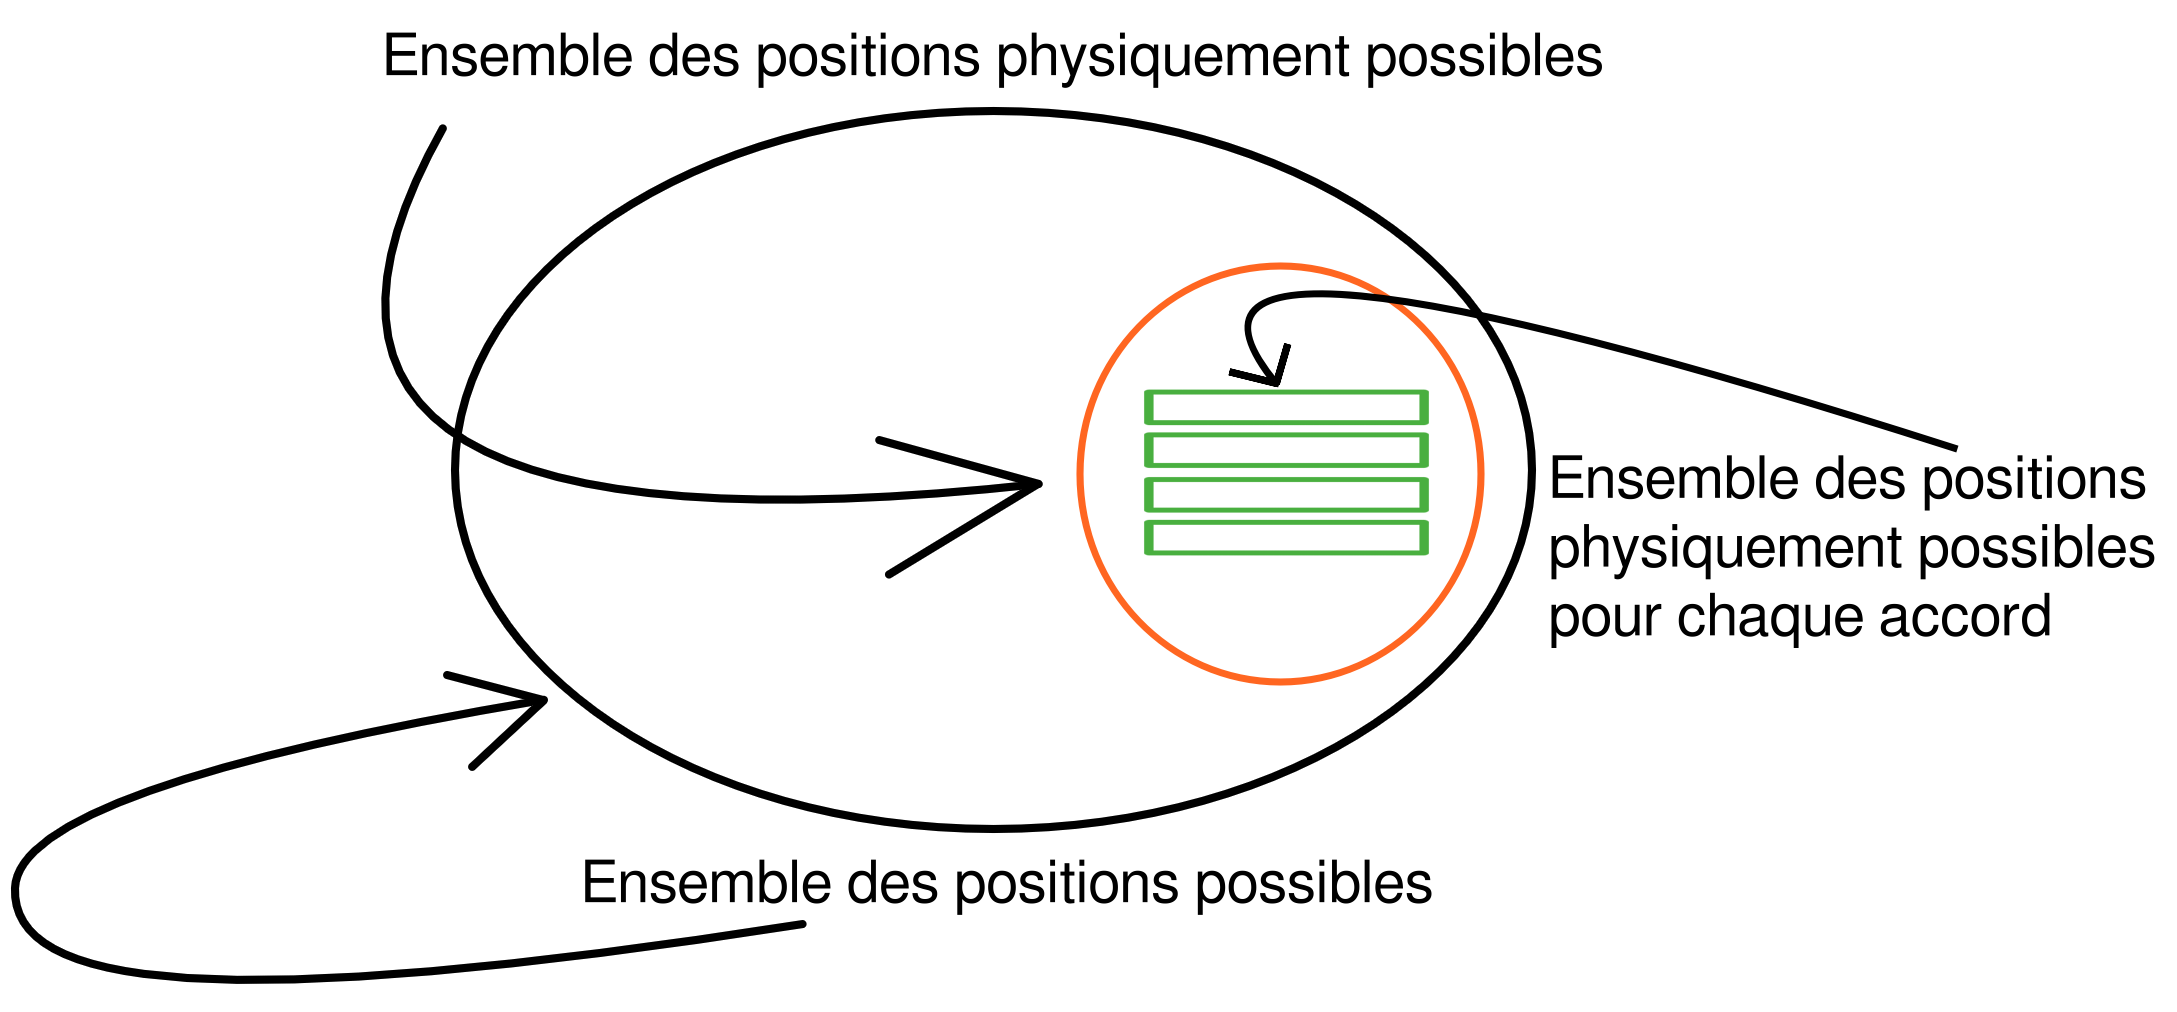
\includegraphics[width=0.5\textwidth]{images/ensembles/ensemble2.png}
  \caption{Représentation de l'affinage du filtrage prenant en compte la nature
  des accords.}
  \label{fig:ensemble2}
\end{figure}

Comme représenté dans la figure \ref{fig:ensemble2}, on obtient un plus grand
nombre de tables mais toutes restreintes à l'essentiel. En effet, elles
comportent uniquement les positions pertinentes.
On aura alors un espace de recherche de taille
$\displaystyle\prod_{i=0}^{\nbAccord}|\ttt{table}.get(\accord[i])|$. 
Finalement, compte tenu de la taille des tables, la taille de l'espace de
recherche est très inferieure à celle de l'ensemble des positions phyisquement 
jouables.

Une fois cela implémenté, on obtient un algorithme plus performant.
On observe qu'en ajoutant le processus de transformation en SAC, on ne gagne
pas en rapidité. Le prétraitement s'effectue très rapidement. On en conclut
qu'il n'y a que très peu de domaines raffinés par le pré-processing SAC dans 
cette modélisation du problème et qu'il n'est donc plus nécessaire. 
D'une certaine manière, on a réalisé le travail du prétraitement de la SAC
au moment du filtrage. Cela revient à dire que l'on a modélisé le problème de
manière à avoir les domaines les plus petits possibles.

Dans cette modélisation, les seules réelles contraintes indiquées au solver
sont des contraintes d'appartenance des positions à une table, 
et une contrainte de minimisation.
Les contraintes de correspondance position / accord sont inutiles car toutes
les positions du domaine sont des positions correspondant à l'accord demandé.



\subsection{Minimisation et liberté laissée à l'instrumentiste}
\label{subsec:Minimisation}

Le but de ce projet peut être vu de deux manières. D'une part, permettre à des
personnes pour qui la guitare n'est pas l'instrument de prédiléction notamment
des débutants de trouver une suite de doigtés pour une suite d'accords. 
Mais d'un autre côté certains instrumentistes peuvent aussi vouloir utiliser 
cet outil pour trouver des doigtés en fonction de contraintes qu'eux mêmes 
poseraient.
C'est pourquoi, avec l'aide de deux guitaristes, Mikahïl Malt et Cléo Langlois,
nous avons réfléchi à comment donner de la liberté à une personne utilisant
cet outil.

\subsubsection{Personnalisation}
\label{subsubsec:Personalisation}

Nous avons donc réalisé une section préference dans la classe définissant
l'instumentiste. Dans cette section, on peut renseigner différents critères :

\begin{itemize}
\label{list:preferences}
  \item Avoir les positions les plus proches d'une certaine frette
  \item Jouer la note fondamentale de l'accord à la basse
  \item Avoir le moins de cordes non jouées
  \item Avoir le moins de cordes à vide car le son d'une telle corde est 
    moins joli
  \item Avoir une distance minimale entre les positions adjacentes
    temporellement
  \item Eviter de jouer deux fois des notes de même fréquence (dans le cas où
    il y aurait un désaccordage même léger de l'instrument, il peut y avoir un
    problème de phase entre ces différents sons).
\end{itemize}

Pour chaque critère, soit il est fixé et on élimine dans le filtrage toutes les 
positions qui ne répondent pas au critère qui est exprimé avec un système de 
bornes, soit il est laissé à la minimisation dans ce cas avec un poids associé.
On peut alors définir des profils, par exemple celui d'une personne 
débutante qui préfèrera rester en haut du manche, avoir le plus de cordes à 
vide et changer de position le moins possible. On peut aussi laisser libre 
cours à l'imagination de l'instrumentiste.

\subsubsection{Fonction de minimisation}
\label{subsubsec:funMinimisation}

La fonction de minimisation est une fonction qui renvoie une indéterminé et
qui traite d'indéterminées. Il se trouve que faire des manipulations
arithmétiques et des tests sur les valeurs des indéterminées c'est assez
compliqué. Par exemple, une fonction que j'ai beaucoup utilisée est la
suivante:

\[
  \begin{array}{l|rcl}
    f : & \mathbb{Z} & \longrightarrow & \left\{ 0, 1\right\} \\
        & n & \longmapsto & \frac{1+\frac{n-\lvert n-1\rvert}{\lvert n-\lvert n-1\rvert\rvert}}{2}
  \end{array}
\]

Cette fonction renvoie les entiers strictement positifs sur $1$ et les entiers
négatifs sur $0$. Avec des décalages et des compositions d'elle même, $f$
permet par exemple de compter le nombre de cordes non jouées, de le pondérer
avec le poids associé et de l'ajouter à la quantité à minimiser. 
Dans mon code j'ai appelé cette fonction \ttt{surjectionPositif}.

\begin{figure}[h]
\begin{lstlisting}[language=Java]
if (!player.preferences.cordesNonJoueesFix)
{
	for (int i=0; i<doigtes.length; i++)
	{
		for (int j=0; j<doigtes[i].length; j++)
		{
			res = res.add(((ClasseOutilsMaths.surjectionPositif(model, doigtes[i][j].add(1).intVar())).sub(1)).mul(-1).mul(player.preferences.cordesNonJoueesPoids)).intVar();
		}
	}
}
\end{lstlisting}
  \caption{Exemple d'utilisation de \ttt{surjectionPositif} afin de compter le 
  nombre de cordes non jouées dans la position}
  \label{code:cordesNonJouees}
\end{figure}

Dans le code \ref{code:cordesNonJouees}, chaque corde non jouée dans la
position \ttt{i} provoque un incrément de la quantité à minimiser de 
\ttt{player.preferences.cordesNonJoueesPoids} qui est le poids associé à la 
minimisation du nombre de cordes non jouées défini dans les préférences.

On a construit la fonction à minimiser comme suit :

\begin{lstlisting}[language=Java]
static IntVar fonctionToMinimize(Model model, IntVar[][] doigtes, int nf, int[][] chords, int[] scordature, int[][] parametres)
\end{lstlisting}

Dans la fonction on rentre toutes les informations nécessaires : modèle, les
indéterminées, le nombre de frettes, les accords ...\\
Mais on indique aussi des parametres qui vont pouvoir modifier la
fonction de minimisation.

Les paramètres de préférence sont définis dans la classe \ttt{preference}.
Ils fonctionnent de la sorte :\\
Chaque paramètre listé dans la section \ref{list:preferences} est défini par
plusieurs variables : une variable booléenne définissant si la contrainte est
à fixer ou à minimiser, puis une variable de bornes à utiliser en cas de
contraintes fixes, et un poids et des limites dans le cas de la contrainte de
minimisation.

Voici un tableau listant les paramètres laissés à l'instrumentiste.

\begin{figure}[h]
%\begin{center}
\begin{tabular}{||c c c c||}
 \hline
  Fix & Borne & Limite & Poids\\ [0.5ex]
 \hline\hline
  fretteMoyenneFix & \makecell{fretteMoyenneSup\\fretteMoyenneInf} & fretteMoyenne & fretteMoyennePoids\\
 \hline
  fondaBassFix & / & / & fondaBassPoids \\
 \hline
  cordesNonJoueesFix & cordesNonJoueesMax & / & cordesNonJoueesMax \\
 \hline
  pasRepetitionFix & pasRepetitionMax & / & pasRepetitionPoids \\
 \hline
  cordesAVidesFix & cordesAVidesMax & / & cordesAVidesPoids \\ [1ex]
 \hline
\end{tabular}
%\end{center}
\caption{Tableau des paramètres ajustables par l'instrumentiste}
\label{tabm:Param}
\end{figure}

On peut ainsi modifier la recherche dans la fonction à minimiser, en fonction
des choix de l'instrumentiste.

\subsection{Amélioration}
\label{subsec:amelioration}

Avec mes encadrants et Mikahïl Malt, nous avons considéré plusieurs pistes 
d'amélioration à ce second modèle. D'une part, il peut y avoir des 
améliorations sur le plan algorithmique et l'effeicacité du programme, et de
l'autre, il peut y avoir des améliorations sur le plan des préférences laissées
au guitariste.

\subsubsection{Algorithmique}
\label{subsubsec:Algorithmique}

La fonction à minimiser est une fonction qui prend en entrée des IntVar et qui
renvoie un IntVar. Bien que cela soit possible, traiter des IntVar de manière
arithmétique est assez fastidieux. 
Ainsi, la manière de calculer la fonction de minimisation n'est pas optimale.
Une manière d'améliorer cela serait d'ajouter à l'étape du filtrage des
positions le stockage d'informations par rapport à la position. 
On pourrait stocker toutes les informations nécessaires à la fonction de 
minimisation, comme le nombre de cordes à vide.
Au cours de la fonction de minimisation, on n'aurait plus qu'à récupérer ces 
informations déjà calculées au lieu d'utiliser des expressions arithmétiques
sur des indéterminées.
J'ai commencé à implémenter un tel système mais je n'ai pas pu le finaliser.

\subsubsection{Préférences}
\label{subsubsection:Preferences}

Avec Mikhaïl Malt et Charlotte Truchet, nous avons réfléchi à une manière de
déterminer la position précise des doigts sur le manche. Cela permetterait 
d'indiquer sur la tablature quel doigt poser au lieu d'indiquer où les 
cordes doivent être bloquées. On pourrait aussi ajouter de la liberter
à l'instrumentiste dans les préferences ainsi qu'un confort de lecture.
On pourrait alors avoir une manière plus précise pour déterminer le barré ainsi
qu'une distance entre les doigts plus fine avec la position exacte du doigt.\\
On peut déterminer la position des doigts en considérant l'ordre suivant :
\begin{itemize}
  \item Un premier ordre de l'index à l'auriculaire sur les frettes
    décroissantes.
  \item Un second ordre des cordes graves aux cordes aigües sur la même frette.
\end{itemize}
On peut alors determiner une position précise des doigts sur le manche, mais
cela reste à implémenter.\\
On peut aussi imaginer définir un ensemble de préférences (un par accord) pour
adapter les préférences au cours du morceau.\\
On pourrait définir un durée entre chaque accord, ce qui
permetrait par exemple entre deux accords distants d'une longue periode
temporelle de sectionner la partition et d'opérer le calcul sur des sous suites
d'accords en considérant que l'instrumentiste peut pendant le laps de temps
changer sereinement de position.
Les deux ajouts précédents pourraient, combinés, permettre de définir un modèle
de résolution pour trouver les positions pour une partition et non plus une
suite d'accords.

On pourrait aussi réfléchir à une meilleur modélisation des doigts, vu non pas
de manière abstraite mais basée sur la morphologie des dooigts et de la main.
En reprenant le travail de Leandro Costalonga \cite{biomechanicalCostalonga}, 
on pourrait déterminer de manière plus fiable si une position est jouable ou 
si elle ne l'est pas.
On pourrait aussi ajouter une dimension de fatigue ou de difficultée musculaire
pour le jeu d'un morçeau.
\newpage
